\documentclass[11pt]{article}
\usepackage[margin=1in]{geometry}
\usepackage{graphicx}
\usepackage{booktabs}
\usepackage{hyperref}
\hypersetup{pdftitle={Sorting and Searching, Measured}, pdfauthor={Built by AI agents; see the project repository}, pdfsubject={Counted comparisons and probes for five sorts and three searches, checked against Big O}}
\title{Sorting and Searching, Measured}
\author{Built by AI agents; see the project repository}
\date{}
\begin{document}
\maketitle

\section{What this is}
Five sorting algorithms (bubble, insertion, selection, merge and quick sort) and three searches (linear, binary and recursive binary) are written as small Python classes. Each one counts the work it does: comparisons and moves for sorting, probes for searching. Counting, unlike timing, gives the same answer on every machine, so the measurements can be checked against Big O. Every list is generated from a fixed seed. The source, the result files and the record of how the agents built it are at \url{https://github.com/jeremy-evert/sorting_and_searching}.

\section{Sorting}
Figure~\ref{fig:sort} shows comparisons against list size for random input on logarithmic axes, where a steeper line means faster growth. Bubble and selection sort lie on top of each other and grow as $n^2$; insertion sort is also $n^2$ on random input but with a smaller constant; merge and quick sort grow as $n \log n$ and stay far below.

\begin{figure}[ht]
\centering
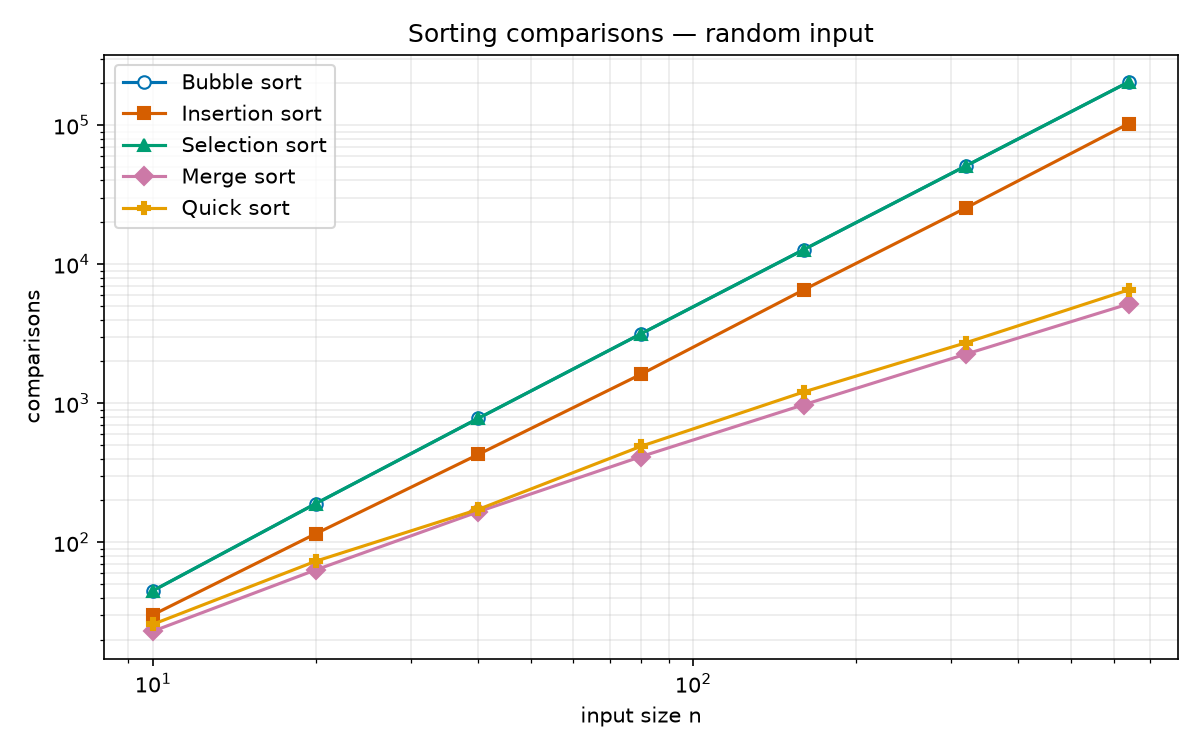
\includegraphics[width=0.9\textwidth]{../docs/plots/sorting_random.png}
\caption{Comparisons against list size, random input.}
\label{fig:sort}
\end{figure}

\section{Searching}
Half of the lookups are for items in the list and half for items that are not. Linear search must look at about half the list for a hit and all of it for a miss, so on average about $3n/4$ items; binary search halves the range each probe and needs about $\log_2 n$.

\begin{figure}[ht]
\centering
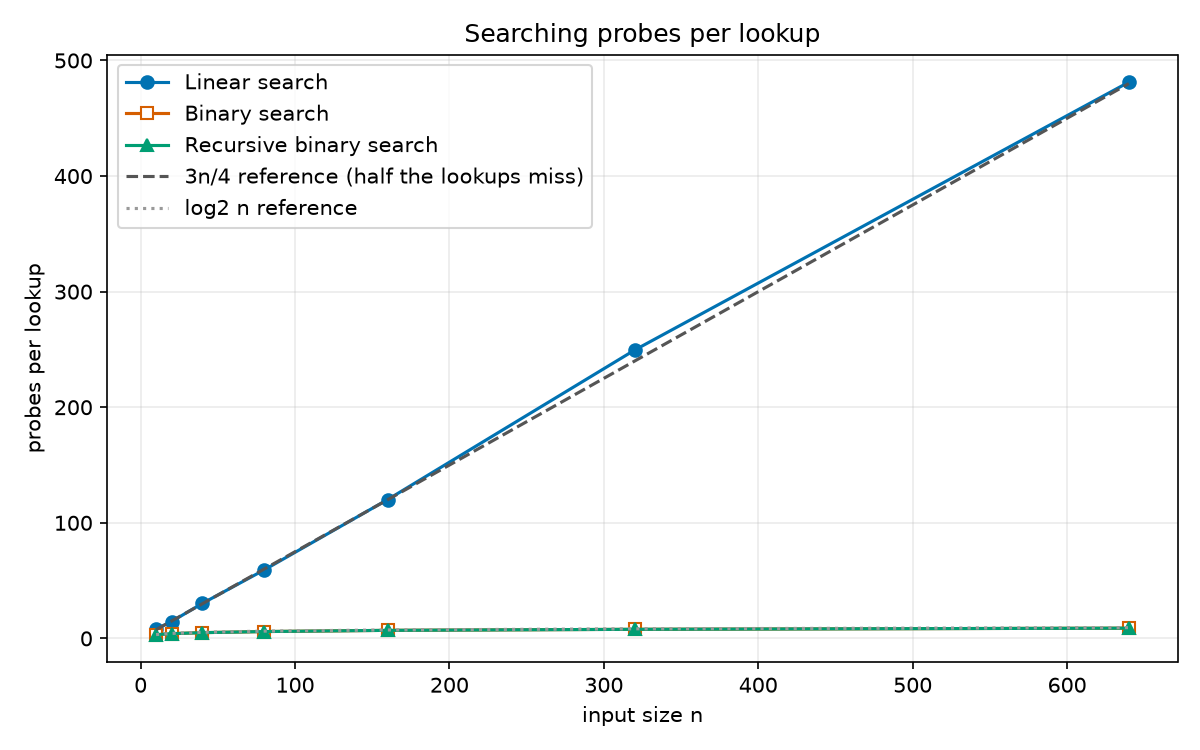
\includegraphics[width=0.9\textwidth]{../docs/plots/searching.png}
\caption{Probes per lookup against list size, with the $3n/4$ and $\log_2 n$ reference lines.}
\label{fig:search}
\end{figure}

\section{Does the theory match?}
The \emph{doubling question} asks how much more work a list twice as long costs: about $2\times$ for $n$, a little over $2\times$ for $n \log n$ (2.24 between sizes 320 and 640), and $4\times$ for $n^2$. Tables~\ref{tab:sort} and~\ref{tab:search} compare prediction with measurement; they are the same tables as in \texttt{BIG\_O.md}, which a script checks against the data. The ratio is comparisons at size 640 divided by comparisons at size 320.

\begin{table}[ht]
\centering
\small
\begin{tabular}{llllrrrl}
\toprule
input & sorter & predicted & pred.\ ratio & at 320 & at 640 & ratio & agrees \\
\midrule
random & bubble & n\^{}2 & 4.00 & 51040.0 & 204480.0 & 4.01 & yes \\
random & insertion & n\^{}2 & 4.00 & 25451.8 & 102692.0 & 4.03 & yes \\
random & selection & n\^{}2 & 4.00 & 51040.0 & 204480.0 & 4.01 & yes \\
random & merge & n log n & 2.24 & 2259.8 & 5182.8 & 2.29 & yes \\
random & quick & n log n & 2.24 & 2727.6 & 6544.8 & 2.40 & no \\
sorted & bubble & n\^{}2 & 4.00 & 51040.0 & 204480.0 & 4.01 & yes \\
sorted & insertion & n & 2.00 & 319.0 & 639.0 & 2.00 & yes \\
sorted & selection & n\^{}2 & 4.00 & 51040.0 & 204480.0 & 4.01 & yes \\
sorted & merge & n log n & 2.24 & 1280.0 & 2880.0 & 2.25 & yes \\
sorted & quick & n\^{}2 & 4.00 & 51040.0 & 204480.0 & 4.01 & yes \\
reversed & bubble & n\^{}2 & 4.00 & 51040.0 & 204480.0 & 4.01 & yes \\
reversed & insertion & n\^{}2 & 4.00 & 51040.0 & 204480.0 & 4.01 & yes \\
reversed & selection & n\^{}2 & 4.00 & 51040.0 & 204480.0 & 4.01 & yes \\
reversed & merge & n log n & 2.24 & 1408.0 & 3136.0 & 2.23 & yes \\
reversed & quick & n\^{}2 & 4.00 & 51040.0 & 204480.0 & 4.01 & yes \\
\bottomrule
\end{tabular}
\caption{Sorting comparisons and doubling ratios.}
\label{tab:sort}
\end{table}

\begin{table}[ht]
\centering
\small
\begin{tabular}{llrrrr}
\toprule
searcher & predicted & pred.\ at 320 & pred.\ at 640 & probes at 320 & probes at 640 \\
\midrule
linear & 3n/4 & 240.00 & 480.00 & 249.50 & 481.25 \\
binary & log2 n & 8.32 & 9.32 & 7.87 & 8.88 \\
recursive binary & log2 n & 8.32 & 9.32 & 7.87 & 8.88 \\
\bottomrule
\end{tabular}
\caption{Searching probes per lookup.}
\label{tab:search}
\end{table}

\section{Discussion}
Most rows agree with theory. The interesting rows are the ones that appear to differ.

\paragraph{Insertion sort on sorted input is linear.} Each item is compared once with its left neighbour and stays put: 639 comparisons at size 640.

\paragraph{Quick sort on sorted input is $n^2$.} The implementation uses the first item as the pivot on purpose. On sorted input that pivot is always the smallest item, so each round removes one item and the comparison count equals bubble sort's, 204480 at size 640.

\paragraph{Quick sort on random input} shows a ratio of 2.40 against a predicted 2.24 and is marked ``no'' in the table. It is clearly still $n \log n$, not $n^2$. We tested the explanation: with 500 random lists per size the ratio is 2.31, and the exact expected count for a first-item pivot, $2(n+1)H_n-4n$, gives 2.313. So the five-list average was unlucky, and the rest of the gap is the lower-order terms, which fade only slowly as $n$ grows.

\paragraph{Merge sort} has a ratio a little above 2 because doubling the list also adds a level of splitting.

\paragraph{Search.} Linear search averages about $3n/4$ probes, not $n/2$, because misses cost the full $n$. Binary search sits slightly under $\log_2 n$ because hits are found before the last halving; from size 320 to 640 it rises by one probe, as a $\log n$ curve should.

\paragraph{In practice.} At a million items, $n \log n$ is about 20 million comparisons while $n^2/2$ is about five hundred billion, roughly 25{,}000 times more; at a billion comparisons per second that is a fiftieth of a second against about eight minutes.

\end{document}
